%%%%%% -*- Coding: utf-8-unix; Mode: latex

%\documentclass[polish]{projectreport}
\documentclass[english]{projectreport}

\usepackage[utf8]{inputenc}
\usepackage{url}
\usepackage{subfigure}
\usepackage{tabularx}
\usepackage{ragged2e}
\usepackage{booktabs}
\usepackage{multirow}
\usepackage{grffile}
\usepackage{float}

\usepackage[bookmarks=false]{hyperref}
\hypersetup{colorlinks,
  linkcolor=blue,
  citecolor=blue,
  urlcolor=blue}

\usepackage{indentfirst}
\usepackage{caption}
\usepackage{listings}
\usepackage[ruled,linesnumbered,lined]{algorithm2e}
\usepackage[svgnames]{xcolor}
\usepackage{inconsolata}
\usepackage{fancyhdr}

\usepackage{csquotes}
\DeclareQuoteStyle[quotes]{polish}
  {\quotedblbase}
  {\textquotedblright}
  [0.05em]
  {\quotesinglbase}
  {\fixligatures\textquoteright}
\DeclareQuoteAlias[quotes]{polish}{polish}

\usepackage[
style=numeric,
sorting=nyt,
isbn=false,
doi=true,
url=true,
backref=false,
backrefstyle=none,
maxnames=10,
giveninits=true,
abbreviate=true,
defernumbers=false,
backend=biber]{biblatex}
\addbibresource{bibliography.bib}

\lstset{
    %language=Python, %% PHP, C, Java, etc.
    basicstyle=\ttfamily\footnotesize,
    backgroundcolor=\color{gray!5},
    commentstyle=\it\color{Green},
    keywordstyle=\color{Red},
    stringstyle=\color{Blue},
    numberstyle=\tiny\color{Black},    
    % morekeywords={TestKeyword},
    % mathescape=true,
    escapeinside=`',
    frame=single, %shadowbox, 
    tabsize=2,
    rulecolor=\color{black!30},
    title=\lstname,
    breaklines=true,
    breakatwhitespace=true,
    framextopmargin=2pt,
    framexbottommargin=2pt,
    extendedchars=false,
    captionpos=b,
    abovecaptionskip=5pt,
    keepspaces=true,            
    numbers=left,                    
    numbersep=5pt,                  
    showspaces=false,                
    showstringspaces=false,
    showtabs=false,
    tabsize=2
}

\SetAlgorithmName{\LangAlgorithm}{\LangAlgorithmRef}{\LangListOfAlgorithms}

\renewcommand{\lstlistingname}{\LangListing}
\renewcommand\lstlistlistingname{\LangListOfListings}

\newcolumntype{Y}{>{\small\centering\arraybackslash}X}
%\newcolumntype{b}{>{\hsize=1.6\hsize}Y}
%\newcolumntype{m}{>{\hsize=.6\hsize}Y}
%\newcolumntype{s}{>{\hsize=.4\hsize}Y}

\captionsetup[figure]{skip=5pt,position=bottom}
\captionsetup[table]{skip=5pt,position=top}



%%%%%%%%%%%%%%%%%%%%%%%%%%%%%%%%%%%%%%%%%%%%%%%%%%%%%%%%%%%%%%%%%%%%%%%%%%%%%%%
\author{Jakub Karczewski \and Wojciech Fortuna}

\title{Simulation of a team of drones using the Webots simulator}

\date{13.05.2026}
      
\pagestyle{fancy}
\fancyhf{}
\fancyhead[LE,RO]{\thepage}

%%%%%%%%%%%%%%%%%%%%%%%%%%%%%%%%%%%%%%%%%%%%%%%%%%%%%%%%%%%%%%%%%%%%%%%%%%%%%%%
\begin{document}

\maketitle

\thispagestyle{empty}

%\begin{abstract}
%\noindent Abstract of the paper
  
%\noindent\textbf{Keywords:} evolutionary algorithms, neural networks
%\end{abstract}

\begin{abstract}
\noindent
This report presents a simulation framework for multi-drone search and rescue
missions in terrain with non-uniform elevation. The considered problem assumes
that the target position is unknown and represented by a probability map over
the search area. Drone detection depends on both sensor range and terrain-based
line-of-sight visibility. The project implements two trajectory planning
approaches: a greedy multi-drone planner and a genetic algorithm. The proposed
methods are evaluated using batch experiments that compare coverage, travelled
distance, search efficiency, and expected target detection time under different
mission parameters. The results show how the number of drones, detection radius,
time budget, deployment pattern, probability map, and terrain difficulty affect
the quality of the generated search trajectories.

\noindent\textbf{Keywords:} multi-drone search, search and rescue, Webots,
trajectory planning, genetic algorithm, greedy algorithm, expected detection time
\end{abstract}


\section{Introduction and review of related research}

\subsection{Domain analysis}

Search and rescue (SAR) operations are conducted in order to locate and assist
missing persons in potentially dangerous environments. One of the most
challenging scenarios for such operations is mountainous terrain.

Mountain regions are characterized by complex topography, including ridges,
valleys and steep slopes. These features significantly limit accessibility
and visibility. Ground-based search is often slow, physically demanding,
and sometimes even dangerous for rescue teams. Additionally, environmental
conditions such as weather, vegetation, and lack of infrastructure may further
hinder the search process.

In mountainous areas, even relatively short distances on a map may correspond
to difficult or impassable routes in practice. This makes systematic search
particularly challenging and often requires dividing the terrain into smaller
regions that can be explored independently.

Time plays a crucial role in search and rescue missions. The probability of
finding a missing person decreases with time, which makes efficient search
strategies extremely important. In many real-world cases, the first few hours
of the search are the most critical.

In recent years, unmanned aerial vehicles (UAVs), commonly referred to as
drones, have been increasingly used to support search operations. As shown
in \cite{goodrich2008uav}, drones allow fast exploration of large areas and can access locations
that are difficult to reach by humans.

Compared to ground-based methods, UAVs can significantly reduce the time
required to scan large areas. They can also be deployed quickly and operate
independently of road infrastructure. This makes them particularly useful
in emergency situations.

However, the use of drones does not eliminate all challenges. One of the
key limitations is restricted visibility caused by terrain. Even though
drones operate in three-dimensional space, their sensors are often unable
to detect objects hidden behind terrain obstacles such as hills or ridges.
In practice, this means that even relatively close locations may remain
unobserved due to terrain occlusions.

As a result, planning effective search trajectories becomes a non-trivial task,
especially when multiple drones are involved.

\subsection{Problem analysis}

The main problem considered in this work is the coordination of multiple
drones performing a search task in a mountainous environment.

The environment is represented by a terrain model, where elevation varies
across the area. The terrain model is assumed to be known in advance. This
means that all geometric properties of the environment, including elevation
and visibility relations, are available before trajectory planning begins.

This allows the problem to be formulated as an offline planning task, where
trajectories are computed based on complete knowledge of the environment.

Visibility between two points depends on the terrain shape. The importance
of such visibility constraints has been discussed in computational geometry \cite{deberg2008cg}.
In practice, this implies that the ability of a drone to observe a region
cannot be determined solely based on distance.

The searched person is assumed to be located at an unknown position.
Instead of a deterministic location, the position is modeled using a
probability distribution over the terrain. This approach is commonly used
in search theory \cite{stone1975search} and allows incorporating prior knowledge about the
likely location of the target.

For example, certain regions may be considered more probable than others
due to terrain characteristics, accessibility, or last known position
of the missing person.

Each drone follows a predefined trajectory. During the mission, drones do
not change their behavior or adapt to new information. This assumption
simplifies the problem and allows focusing on the quality of trajectory
planning. As a consequence, the effectiveness of the search depends entirely
on how well the trajectories are designed before the mission.

Detection of the target depends on two main factors: distance and visibility.
A drone can detect the target only if it is sufficiently close and if there
are no terrain obstacles blocking the line-of-sight.

This makes the problem inherently three-dimensional and strongly dependent
on terrain geometry. In particular, the same trajectory may be effective
in one region of the terrain and ineffective in another.

The goal of the problem is to design trajectories for multiple drones such
that the expected time required to detect the target is minimized.

\subsection{Related approaches}

The described problem is related to several research areas, including
coverage path planning, probabilistic search, and multi-agent systems.

Coverage path planning focuses on systematic exploration of a given region.
As discussed in \cite{choset2001coverage}, classical approaches such as grid-based methods and
sweeping patterns are effective when the objective is to ensure complete
coverage of the environment.

However, in the considered problem, full uniform coverage is not the primary
goal. Instead, the objective is to minimize the expected detection time of
a target whose location is described by a probability distribution.
Consequently, different regions of the terrain have different importance,
and uniform coverage strategies may be inefficient if they do not prioritize
high-probability areas. Moreover, detection depends not only on visiting
a region, but also on distance and line-of-sight conditions.

Another important area is probabilistic search, where the target location is
modeled using a probability distribution \cite{stone1975search}. In such approaches, search
strategies are designed to prioritize regions with higher likelihood of
containing the target. This aligns more closely with the objective considered
in this work.

However, many probabilistic search models assume simplified sensing conditions
or do not explicitly account for terrain-dependent visibility. In the presence of terrain obstacles, visiting a region does not necessarily
imply that the target can be detected. Detection depends explicitly on
distance and line-of-sight conditions, which must be satisfied simultaneously.

Coordination of multiple agents in search and coverage tasks has also been
widely studied. For example, \cite{schwager2011distributed} investigates distributed control strategies
for multi-robot systems. The use of multiple drones allows parallel
exploration of the environment, which can significantly reduce search time.

At the same time, multi-agent coordination introduces additional challenges,
such as avoiding redundant coverage and ensuring efficient allocation of
search effort between agents.

In summary, each of the discussed approaches addresses a different aspect
of the problem, including coverage, uncertainty, and multi-agent coordination.

\subsection{Research goals}

The objective of this project is to analyze and simulate the problem of
coordinated search using a team of drones in a three-dimensional terrain.

The main goals of the project are:

\begin{itemize}
    \item to model the search environment using a terrain representation,
    \item to incorporate visibility constraints resulting from terrain geometry,
    \item to model uncertainty of the target location,
    \item to design trajectory planning strategies for multiple drones,
    \item to minimize the expected detection time,
    \item to evaluate the approach in a simulation environment.
\end{itemize}

\section{Problem formulation and proposed solution}

In this section, a formal model of the considered multi-drone search problem is introduced. The formulation includes the terrain representation, the drone motion model, the probabilistic description of the target location, and the detection conditions.

Based on these components, the objective function is defined as the expected detection time. The problem is treated as an offline trajectory planning task under geometric and kinematic constraints.

\subsection{Problem formulation}

\subsubsection{Environment model}

The environment is represented by a three-dimensional terrain model given in the form of a height function
\begin{equation}
h : \mathbb{R}^2 \rightarrow \mathbb{R}.
\end{equation}

For any horizontal position $(x, y) \in \mathbb{R}^2$, the value $h(x, y)$ defines the elevation of the terrain at that point.

The terrain model is assumed to be known before the planning stage. This allows determining geometric properties of the environment, including visibility relations between points in space.

In particular, visibility between two points depends on whether the line segment connecting them intersects the terrain surface.

\subsubsection{Drone model}

A team of $N$ drones is considered. Each drone $i \in \{1, \dots, N\}$ is described by its trajectory
\begin{equation}
x_i(t) \in \mathbb{R}^3, \quad t \in [0, T],
\end{equation}
where $T$ denotes the time horizon of the mission.

Each drone is assigned an initial position
\begin{equation}
x_i(0) = x_i^0 \in \mathbb{R}^3,
\end{equation}
which is known and fixed before the mission begins.

The motion of each drone is subject to kinematic constraints. In particular, the velocity is bounded by
\begin{equation}
\|\dot{x}_i(t)\| \leq v_{\max}, \quad \forall t \in [0, T].
\end{equation}

Additionally, drones operate above the terrain surface, which implies
\begin{equation}
z_i(t) \geq h(x_i(t), y_i(t)).
\end{equation}

Trajectories are planned offline and remain fixed during the mission.

\subsubsection{Detection model}

Detection of the target depends on both distance and visibility.

Let $x_i(t)$ denote the position of drone $i$ at time $t$. The detection function is defined as
\begin{equation}
D_i(t, y) =
\begin{cases}
1 & \text{if } \|x_i(t) - y\| < d_{\max} \ \land \ \mathrm{LoS}(x_i(t), y) = 1, \\
0 & \text{otherwise}.
\end{cases}
\end{equation}

The function $\mathrm{LoS}(x, y)$ indicates whether there exists a direct line-of-sight between positions $x$ and $y$, i.e., whether the line segment connecting them is not obstructed by the terrain.

\subsubsection{Detection time}

For a given target position $y$, the detection time is defined as
\begin{equation}
T(y) = \min \left\{ t \geq 0 : \exists i \in \{1, \dots, N\}, \ D_i(t, y) = 1 \right\}.
\end{equation}

If the target is not detected within the time horizon $T$, the detection time is set to $T$.

\subsubsection{Objective function}

The objective of the problem is to minimize the expected detection time over all possible target locations. Formally, this is expressed as
\begin{equation}
\min_{\{x_i(t)\}} \ \mathbb{E}_{y \sim p(y)} \left[ T(y) \right].
\end{equation}

The objective function serves as the main performance measure used to evaluate the quality of planned trajectories.

\subsection{Proposed algorithms}

In order to address the trajectory planning problem formulated above, two complementary algorithms are proposed. The first one is a greedy constructive method that generates feasible trajectories based on local utility. The second one is a genetic algorithm that performs global optimization over the space of multi-drone trajectories.

The combination of these two approaches allows both efficient initialization and further improvement of solution quality.

\subsubsection{Greedy multi-drone trajectory planning}

The first proposed method is a greedy algorithm that incrementally constructs trajectories for all drones. The main idea is to iteratively select observation points that maximize the ratio of expected information gain to travel time.

\paragraph{Discretization}

The continuous terrain is discretized into a finite set of cells
\[
G = \{c_1, c_2, \dots, c_M\},
\]
where each cell \(c_j\) is associated with a probability \(p_j\) of containing the target.

Additionally, a finite set of candidate observation points is defined:
\[
V = \{v_1, v_2, \dots, v_K\}.
\]

For each observation point \(v_k\), a visibility set \(S_k \subseteq G\) is precomputed, containing all cells that can be detected from \(v_k\), taking into account both distance constraints and line-of-sight conditions.

\paragraph{Utility function}

At each step, the algorithm evaluates candidate observation points based on their marginal contribution.

Let \(U \subseteq G\) denote the set of cells that have not yet been observed. For a drone currently located at position \(u\), the travel time to a candidate point \(v\) is defined as
\[
\tau(u, v) = \frac{\|u - v\|}{v_{\max}}.
\]

The marginal gain of visiting point \(v\) is defined as
\[
\Delta(v) = \sum_{c_j \in S_v \cap U} p_j,
\]
which represents the total probability mass of newly observable cells.

The selection criterion is given by
\[
\mathrm{score}(v) = \frac{\Delta(v)}{\tau(u, v) + \varepsilon},
\]
where \(\varepsilon > 0\) is a small constant to avoid division by zero.

\paragraph{Algorithm description}

The algorithm operates iteratively over all drones. At each iteration, it selects the drone and observation point that maximize the score function.

Formally, the following pair is selected:
\[
(i^*, v^*) = \arg\max_{i, v} \mathrm{score}_i(v),
\]
subject to feasibility constraints, such as the remaining time budget.

After selecting the best move:
\begin{itemize}
    \item the observation point \(v^*\) is appended to the trajectory of drone \(i^*\),
    \item the drone's position and time are updated,
    \item all cells in \(S_{v^*}\) are removed from the set \(U\).
\end{itemize}

The process continues until no further feasible moves are possible.

\paragraph{Discussion}

The greedy algorithm is computationally efficient and naturally prioritizes regions with high probability of containing the target. It also avoids redundant coverage by removing already observed cells from consideration.

However, due to its myopic nature, the algorithm may produce suboptimal solutions, especially in complex terrains where long-term planning is required. For this reason, it is used primarily as a baseline method and as an initialization for further optimization.

\subsubsection{Genetic algorithm for trajectory optimization}

To improve upon the solutions generated by the greedy method, a genetic algorithm (GA) is proposed. The GA performs a global search over the space of possible multi-drone trajectories.

\paragraph{Solution representation}

Each individual in the population represents a complete set of trajectories for all drones. A solution is encoded as a sequence of observation points with an assignment to drones:
\[
\pi = \{(v_{1}, i_{1}), (v_{2}, i_{2}), \dots, (v_{L}, i_{L})\},
\]
where \(v_k \in V\) and \(i_k \in \{1, \dots, N\}\) indicates the drone assigned to the observation point.

The order of elements determines the sequence in which observation points are visited.

\paragraph{Fitness function}

The fitness of an individual is defined based on the expected detection time. For each cell \(c_j\), the time of first observation \(t(c_j)\) is determined from the trajectories.

The objective function is given by
\[
J = \sum_{j=1}^{M} p_j \, t(c_j),
\]
which corresponds to the expected detection time.

The fitness function used in the genetic algorithm is defined as
\[
f = -J,
\]
so that lower detection times correspond to higher fitness values.

\paragraph{Initialization}

The initial population consists of:
\begin{itemize}
    \item solutions generated by the greedy algorithm,
    \item randomly generated solutions,
    \item perturbed versions of greedy solutions.
\end{itemize}

This hybrid initialization improves both solution quality and population diversity.

\paragraph{Genetic operators}

The following operators are used to evolve the population.

\subparagraph{Mutation}

Mutation introduces local modifications to trajectories. The following mutation types are considered:
\begin{itemize}
    \item swapping two observation points,
    \item reassigning a point to a different drone,
    \item inserting a new observation point,
    \item removing an existing point,
    \item reversing a segment of a trajectory.
\end{itemize}

These operations allow exploration of the solution space while preserving feasibility.

\subparagraph{Crossover}

Crossover combines parts of two parent solutions to produce offspring. A simple segment-based crossover is used:
\begin{itemize}
    \item a subsequence of observation points is selected from one parent,
    \item the remaining points are filled using the second parent while preserving order.
\end{itemize}

\paragraph{Constraint handling}

After each genetic operation, solutions are checked for feasibility. If necessary, repair procedures are applied:
\begin{itemize}
    \item trajectories exceeding the time horizon are truncated,
    \item infeasible transitions are removed or corrected.
\end{itemize}

\paragraph{Algorithm procedure}

The genetic algorithm follows the standard evolutionary scheme:
\begin{enumerate}
    \item initialize population,
    \item evaluate fitness of all individuals,
    \item repeat until termination:
    \begin{itemize}
        \item select parents,
        \item apply crossover and mutation,
        \item repair infeasible solutions,
        \item evaluate offspring,
        \item update population.
    \end{itemize}
\end{enumerate}

\paragraph{Discussion}

The genetic algorithm enables exploration of a large and complex solution space and can significantly improve upon greedy solutions. It is particularly suitable for multi-drone coordination, as it naturally handles assignment and ordering decisions.

However, it is computationally more expensive than the greedy approach and requires careful design of representation and operators.


\subsection{Simulation model and implementation}

This section describes the developed simulation model and the main software components used in the implementation of the multi-drone search system.

\subsubsection{Simulation environment}

The simulation environment was implemented using the Webots simulator. Webots provides a three-dimensional environment with support for programmable robot controllers, scene modeling, and visualization of autonomous agents.

The project uses a minimal Webots world stored in the \texttt{worlds} directory. The simulation world contains the terrain representation and drone objects used to execute generated waypoint trajectories. The Webots-specific controller is placed in a separate controller directory, following the structure required by Webots.

The trajectory planning modules operate outside the simulator and generate waypoint sequences using the terrain model, probability map, visibility model, and selected planning algorithm. The generated trajectories are exported to a JSON file and then loaded by the Webots drone controller.

The communication between the planning framework and the Webots simulation is therefore file-based. The generated trajectory file has the following structure:
\[
\{
\texttt{"drone\_0"} : [[x_1,y_1,z_1], [x_2,y_2,z_2], \dots]
\}
\]
with analogous entries for additional drones.

During simulation, each drone follows the assigned sequence of waypoints. After reaching a waypoint within a predefined tolerance, the controller switches to the next point. This provides a simple execution layer for trajectories generated by the greedy planner or the genetic algorithm.

The current Webots integration is intentionally minimal and focuses on validating the simulation framework rather than conducting experimental evaluation. Detailed comparisons of trajectory planning methods are left for the experimental part of the report.

\subsubsection{Terrain representation}

The environment is represented using a continuous terrain height function
\[
h(x,y),
\]
which defines terrain elevation for every horizontal position $(x,y)$.

For simulation purposes, the terrain is discretized into a finite grid of cells. Each cell stores:
\begin{itemize}
    \item horizontal coordinates,
    \item terrain elevation,
    \item target probability value.
\end{itemize}

The current implementation uses synthetic mountainous terrain generated from smooth analytical elevation functions.

The discretized terrain representation simplifies visibility analysis, probability modeling, and trajectory planning.

In addition to the internal terrain representation used by the planning algorithms, the generated terrain is also synchronized with the Webots simulation environment in order to provide consistent three-dimensional visualization of the search area.

The terrain geometry is automatically exported from the Python simulation layer to a dedicated Webots PROTO object represented as a polygonal mesh. The current implementation uses an \texttt{IndexedFaceSet} mesh representation to ensure proper compatibility with the Webots rendering system and coordinate conventions.

Terrain coordinates are converted from the internal simulation representation:
\[
[x, y, h(x,y)]
\]
to the Webots coordinate convention:
\[
[x, h(x,y), y].
\]

This approach allows the trajectory planning algorithms, visibility analysis modules, and Webots visualization layer to operate on geometrically consistent terrain representations.

\subsubsection{Visibility model}

One of the key aspects of the considered problem is terrain-dependent visibility.

Visibility between a drone and a target position is evaluated using a line-of-sight (LoS) model.

The visibility condition is approximated by sampling intermediate points along the line segment connecting the drone and the target. For every sampled point, terrain elevation is compared with the altitude of the visibility ray.

If the terrain intersects the viewing ray at any sampled point, the target is considered invisible.

Formally, visibility is defined as
\[
\mathrm{LoS}(x,y)=1
\]
when the line segment connecting positions $x$ and $y$ is not obstructed by terrain.

This approach provides a computationally efficient approximation of terrain-aware visibility.

\subsubsection{Detection model}

Detection depends on both distance and visibility conditions.

A target can be detected only if:
\begin{itemize}
    \item the target remains within the detection radius,
    \item direct line-of-sight exists between the drone and the target.
\end{itemize}

The target position is modeled slightly above the terrain surface in order to simulate a standing person and avoid numerical issues related to terrain intersection.

\subsubsection{Probability map}

The uncertainty of the target location is represented using a probability distribution over the terrain grid.

Each terrain cell is assigned a probability value describing the likelihood of the target being located in that region.

In the current implementation, the distribution is generated using Gaussian hotspots centered around selected terrain regions. This allows modeling prior information about likely target locations.

The probabilities are normalized such that
\[
\sum_{j=1}^{M} p_j = 1.
\]

\subsubsection{Trajectory planning implementation}

The current implementation includes a trajectory planning framework for cooperative multi-drone search operations.

The environment is discretized into:
\begin{itemize}
    \item terrain cells,
    \item candidate observation points.
\end{itemize}

For every candidate observation point, a visibility set is precomputed:
\[
S_k \subseteq G,
\]
where $S_k$ contains all cells observable from observation point $v_k$.

This preprocessing step significantly reduces the computational cost during trajectory planning.

At the current stage of the project, two trajectory planning approaches have been implemented:
\begin{itemize}
    \item a greedy trajectory planner,
    \item a genetic algorithm for trajectory optimization.
\end{itemize}

The greedy planner iteratively selects observation points maximizing the ratio between:
\begin{itemize}
    \item expected probability gain,
    \item travel cost.
\end{itemize}

Candidate moves are evaluated using the score function
\[
\mathrm{score}(v)=
\frac{\Delta(v)}
{\tau(u,v)+\varepsilon},
\]
where:
\begin{itemize}
    \item $\Delta(v)$ denotes the probability mass of newly observable cells,
    \item $\tau(u,v)$ denotes travel time,
    \item $\varepsilon$ is a small constant preventing division by zero.
\end{itemize}

The current implementation supports both:
\begin{itemize}
    \item single-drone planning,
    \item cooperative multi-drone planning.
\end{itemize}

In the multi-drone setting, all drones share information about already observed cells in order to reduce redundant coverage.

Additionally, a genetic algorithm framework was implemented for optimization of multi-drone trajectories.

In the implemented genetic algorithm, each solution is represented as a chromosome containing a sequence of observation assignments:
\[
(drone\_id,\ candidate\_id),
\]
where each gene specifies which drone visits a selected observation point.

This representation allows simultaneous optimization of:
\begin{itemize}
    \item assignment of observation points to drones,
    \item ordering of observation points,
    \item overall trajectory structure.
\end{itemize}

The initial population is generated randomly from the set of candidate observation points.

The fitness function combines:
\begin{itemize}
    \item covered target probability mass,
    \item travelled distance penalty,
    \item mission time constraints.
\end{itemize}

Solutions violating the time budget constraints are repaired by iteratively removing observation points from the chromosome.

The implemented evolutionary process includes:
\begin{itemize}
    \item tournament selection,
    \item one-point crossover,
    \item mutation of drone assignments and observation points,
    \item elitism preserving the best individuals between generations.
\end{itemize}

The modular architecture of the framework allows further extension with additional optimization methods and more advanced evolutionary operators.

\subsubsection{Mission simulation and Webots integration}

The developed framework includes a lightweight mission simulation and execution layer integrated with the Webots simulator.

The overall system architecture is divided into four main layers:
\begin{itemize}
    \item trajectory planning layer,
    \item mission simulation layer,
    \item execution layer,
    \item visualization layer.
\end{itemize}

The trajectory planning layer operates outside the Webots simulator and is responsible for generating waypoint trajectories using the terrain model, probability map, visibility analysis, and trajectory planning algorithms.

The generated trajectories are exported to external JSON files in the following form:
\[
\{
\texttt{"drone\_0"} : [[x_1,y_1,z_1], [x_2,y_2,z_2], \dots]
\}.
\]

The exported trajectories are then loaded by Webots drone controllers responsible for waypoint execution inside the simulation environment.

The mission simulation layer is implemented using the \texttt{SimulationManager} component. This layer is responsible for:
\begin{itemize}
    \item simulation time management,
    \item updating drone positions,
    \item target detection verification,
    \item tracking observed terrain cells,
    \item mission termination handling.
\end{itemize}

The mission execution process terminates when at least one of the following conditions is satisfied:
\begin{itemize}
    \item the target is detected,
    \item the mission time budget is exceeded,
    \item no significant unexplored probability regions remain,
    \item all generated trajectories are completed.
\end{itemize}

The mission state is synchronized with the Webots execution layer using external JSON status files containing:
\begin{itemize}
    \item mission completion status,
    \item target detection status,
    \item mission termination reason,
    \item mission statistics,
    \item target visualization information.
\end{itemize}

The Webots execution layer is intentionally lightweight. Drone motion is implemented using simplified kinematic waypoint following by directly updating the robot translation field inside the simulator. The current implementation does not include advanced flight dynamics, collision avoidance, low-level quadcopter control, or online replanning mechanisms.

The Webots environment is therefore used primarily as:
\begin{itemize}
    \item a trajectory execution framework,
    \item a visualization environment,
    \item a lightweight mission playback system.
\end{itemize}

The current implementation additionally supports synchronization of the generated terrain geometry with the Webots environment. The terrain generated by the Python simulation layer is automatically exported to a dedicated Webots PROTO object represented as a polygonal mesh.

The simulation environment additionally contains a visual representation of the target object. The true target position is synchronized with Webots using a dedicated target status file and a separate visualization controller responsible for updating the target position inside the simulation environment.

Importantly, the trajectory planning algorithms do not have access to the true target position. The true target location is known only by the mission simulation and visualization layers. This separation preserves the probabilistic nature of the search problem and prevents the planning algorithms from exploiting ground-truth target information.

The implemented integration framework provides a modular connection between the external Python-based planning algorithms and the Webots simulation environment while maintaining low implementation complexity and high extensibility for future development.

\subsubsection{System architecture}

The implemented framework consists of several interconnected modules responsible for terrain generation, probability modeling, visibility evaluation, detection checking, trajectory planning, mission simulation, and visualization.

The terrain model and probability map provide input data for the trajectory planning algorithms. The visibility and detection modules are used to determine which terrain cells can be observed from candidate drone positions.

Based on this information, the trajectory planning layer generates waypoint trajectories for multiple drones. The generated trajectories are exported to external JSON files and executed inside the Webots simulation environment.

The framework additionally includes a mission simulation layer responsible for:
\begin{itemize}
    \item mission time management,
    \item target detection verification,
    \item observed terrain tracking,
    \item mission termination handling.
\end{itemize}

The simulation framework additionally supports synchronization of terrain geometry and target visualization with the Webots environment. Dedicated export modules are used to transfer terrain meshes, drone trajectories, mission status information, and target visualization data between the Python-based simulation layer and the Webots execution layer.

The Webots simulation layer is responsible for:
\begin{itemize}
    \item terrain visualization,
    \item waypoint execution,
    \item drone visualization,
    \item target visualization,
    \item mission playback.
\end{itemize}

The implemented system architecture is illustrated below:

\[
\begin{array}{c}
\text{Terrain generation} \\
\downarrow \\
\text{Probability map} \\
\downarrow \\
\text{Visibility and detection model} \\
\downarrow \\
\text{Trajectory planning layer} \\
\downarrow \\
\text{Trajectory export (JSON)} \\
\downarrow \\
\text{Mission simulation layer} \\
\downarrow \\
\text{Mission and target status export} \\
\downarrow \\
\text{Terrain and target synchronization} \\
\downarrow \\
\text{Webots execution and visualization layer}
\end{array}
\]

The modular architecture simplifies further development of the framework and allows independent extension of the planning, simulation, execution, and visualization components.

\newpage

\subsubsection{Software libraries}

The implementation was developed in Python and uses several software tools and libraries supporting numerical computation, visualization, and simulation.

The following software components were used:
\begin{itemize}
    \item Webots simulator,
    \item Python,
    \item NumPy,
    \item Matplotlib,
    \item built-in Python JSON library.
\end{itemize}

Python was used as the primary programming language for implementing the terrain model, visibility analysis, detection model, probability map representation, and trajectory planning algorithms.

NumPy was used for numerical computations, vector operations, and manipulation of three-dimensional coordinates. Matplotlib was used for visualization, debugging, and generation of plots during the development process.

The Webots simulator was used as the simulation and visualization environment for executing drone trajectories generated by the planning algorithms.

Drone trajectories were exported from the planning layer to the simulation environment using JSON files, enabling lightweight integration between the external Python-based planning framework and the Webots execution layer.

The built-in Python JSON library was used for serialization and exchange of waypoint trajectories between the planning algorithms and the Webots controllers.

\subsection{Algorithm pseudocode}

\begin{algorithm}[H]
\caption{Line-of-sight visibility evaluation}
\KwIn{Drone position $x$, target position $y$, terrain height function $h$, number of samples $K$}
\KwOut{Visibility value $\mathrm{LoS}(x,y)$}

\For{$k \leftarrow 1$ \KwTo $K-1$}{
    $\alpha \leftarrow k / K$\;
    $p \leftarrow (1-\alpha)x + \alpha y$\;
    $z_{\mathrm{terrain}} \leftarrow h(p_x, p_y)$\;

    \If{$z_{\mathrm{terrain}} > p_z$}{
        \Return{$0$}\;
    }
}
\Return{$1$}\;
\end{algorithm}

\begin{algorithm}[H]
\caption{Greedy multi-drone trajectory planning}
\KwIn{Drones initial positions $x_i^0$, candidate observation points $V$, terrain cells $G$, probabilities $p_j$, time horizon $T$}
\KwOut{Trajectories for all drones}

Initialize trajectories with initial drone positions\;
Initialize current drone times $t_i \leftarrow 0$\;
Initialize unobserved cells $U \leftarrow G$\;

\ForEach{candidate observation point $v_k \in V$}{
    Precompute visibility set $S_k$\;
}

\While{$U \neq \emptyset$}{
    $bestScore \leftarrow 0$\;
    $bestMove \leftarrow \emptyset$\;

    \ForEach{drone $i$}{
        \ForEach{candidate observation point $v_k \in V$}{
            Compute travel time $\tau(x_i, v_k)$\;

            \If{$t_i + \tau(x_i, v_k) > T$}{
                continue\;
            }

            $\Delta(v_k) \leftarrow \sum_{c_j \in S_k \cap U} p_j$\;
            $score \leftarrow \frac{\Delta(v_k)}{\tau(x_i, v_k)+\varepsilon}$\;

            \If{$score > bestScore$}{
                $bestScore \leftarrow score$\;
                $bestMove \leftarrow (i, v_k)$\;
            }
        }
    }

    \If{$bestMove = \emptyset$}{
        break\;
    }

    Append selected point to the selected drone trajectory\;
    Update selected drone position and time\;
    Remove newly observed cells from $U$\;
}

\Return{trajectories}\;
\end{algorithm}

\begin{algorithm}[H]
\caption{Multi-drone genetic algorithm}
\KwIn{Drones initial positions $x_i^0$, candidate observation points $V$, visibility sets $S_k$, probabilities $p_j$, population size $P$, number of generations $G$}
\KwOut{Optimized multi-drone trajectories}

Initialize population of $P$ random chromosomes\;

\ForEach{chromosome $\pi$ in population}{
    $\pi \leftarrow \{(i_1,v_1),(i_2,v_2),\dots,(i_L,v_L)\}$\;
}

\For{$g \leftarrow 1$ \KwTo $G$}{

    \ForEach{individual $\pi$ in population}{

        Decode $\pi$ into trajectories for all drones\;

        Repair $\pi$ if any drone exceeds the time horizon\;

        Determine observed cells using visibility sets $S_k$\;

        $P_{\mathrm{cov}} \leftarrow \sum_{c_j \in observed} p_j$\;

        Compute total trajectory distance $d_{\mathrm{total}}$\;

        $fitness(\pi) \leftarrow P_{\mathrm{cov}} - \lambda d_{\mathrm{total}}$\;
    }

    Preserve elite individuals\;

    \While{new population is not full}{

        Select two parents using tournament selection\;

        Apply one-point crossover\;

        Mutate drone assignments or observation points\;

        Repair infeasible offspring\;

        Add offspring to new population\;
    }

    Replace old population with new population\;
}

Return the best chromosome decoded into drone trajectories\;
\end{algorithm}


\section{\SectionTitleExperiments}

This section presents the experimental evaluation of the implemented
multi-drone search framework. The experiments were designed to compare the
behavior of the greedy planner and the genetic algorithm under different
mission parameters and environmental conditions.

The evaluation focuses on the following research questions:
\begin{itemize}
    \item how the number of drones affects search quality,
    \item how the sensor detection radius influences coverage and detection time,
    \item how the available mission time budget changes planner performance,
    \item how deployment patterns affect multi-drone cooperation,
    \item how different probability maps and terrain types influence the results,
    \item how greedy planning compares with genetic optimization.
\end{itemize}

\subsection{Experimental setup}

The batch experiments were executed using the configurable experiment framework
implemented in the \texttt{experiments} package. Each batch configuration defines
a set of parameters, and the experiment runner evaluates all combinations of
these parameters. The results are saved in CSV files and then converted into
comparison plots.

The main experimental configurations include:
\begin{itemize}
    \item \texttt{drones\_count\_study} -- comparison of different fleet sizes,
    \item \texttt{detection\_radius\_study} -- comparison of sensor ranges,
    \item \texttt{time\_budget\_study} -- influence of mission duration,
    \item \texttt{start\_pattern\_study} -- comparison of circular and line deployment,
    \item \texttt{probability\_map\_study} -- comparison of hotspot and uniform probability maps,
    \item \texttt{sensor\_resource\_grid\_study} -- joint analysis of fleet size and sensor radius,
    \item \texttt{terrain\_difficulty\_study} -- comparison of flat, hilly, and mountainous terrain.
\end{itemize}

The experiments use synthetic terrain models and probability distributions
implemented in the project. The default scenario uses a hilly terrain and a
hotspot probability map, where the target is more likely to be located near a
selected region. This setup reflects the practical assumption that prior
information about the missing person's likely location is available.

\subsection{Evaluation metrics}

The following metrics are used to evaluate planned trajectories:
\begin{itemize}
    \item \texttt{coverage} -- fraction or probability mass of terrain cells observed by the drones,
    \item \texttt{expected\_target\_detection\_time} -- expected waiting time until target detection,
    \item \texttt{total\_distance} -- total distance travelled by all drones,
    \item \texttt{coverage\_per\_distance} -- search efficiency expressed as coverage per unit distance,
    \item \texttt{total\_waypoints} -- total number of trajectory points,
    \item \texttt{best\_fitness} -- genetic algorithm objective value.
\end{itemize}

The most important metric for the formulated problem is the expected target
detection time. For every terrain cell, the first time at which any drone can
detect the target from its trajectory is computed. These detection times are
then averaged using the probability map as weights. If a cell is not detected
within the planned mission, its detection time is set to the mission time
budget. Lower values of this metric indicate better search performance.

\subsection{Detection radius study}

The detection radius experiment compares the planners for a fixed number of
three drones and a fixed time budget. The detection radius is varied from small
to larger values. This experiment illustrates the influence of sensor range on
the ability to observe terrain cells.

For small detection radii, the drones are unable to observe a significant
portion of the search area. In this case, coverage remains low and the expected
target detection time approaches the mission time budget. Increasing the
detection radius improves visibility coverage and reduces the expected waiting
time for target detection.

The greedy planner tends to react strongly to increased sensor radius because
each selected observation point can cover more previously unobserved cells. The
genetic algorithm can also benefit from increased radius, but its final result
depends on population diversity and the quality of the evolved chromosome.
The generated comparison plots for this experiment are presented in
Figures~\ref{fig:detection-radius-coverage}--\ref{fig:detection-radius-efficiency}.

\begin{figure}[H]
    \centering
    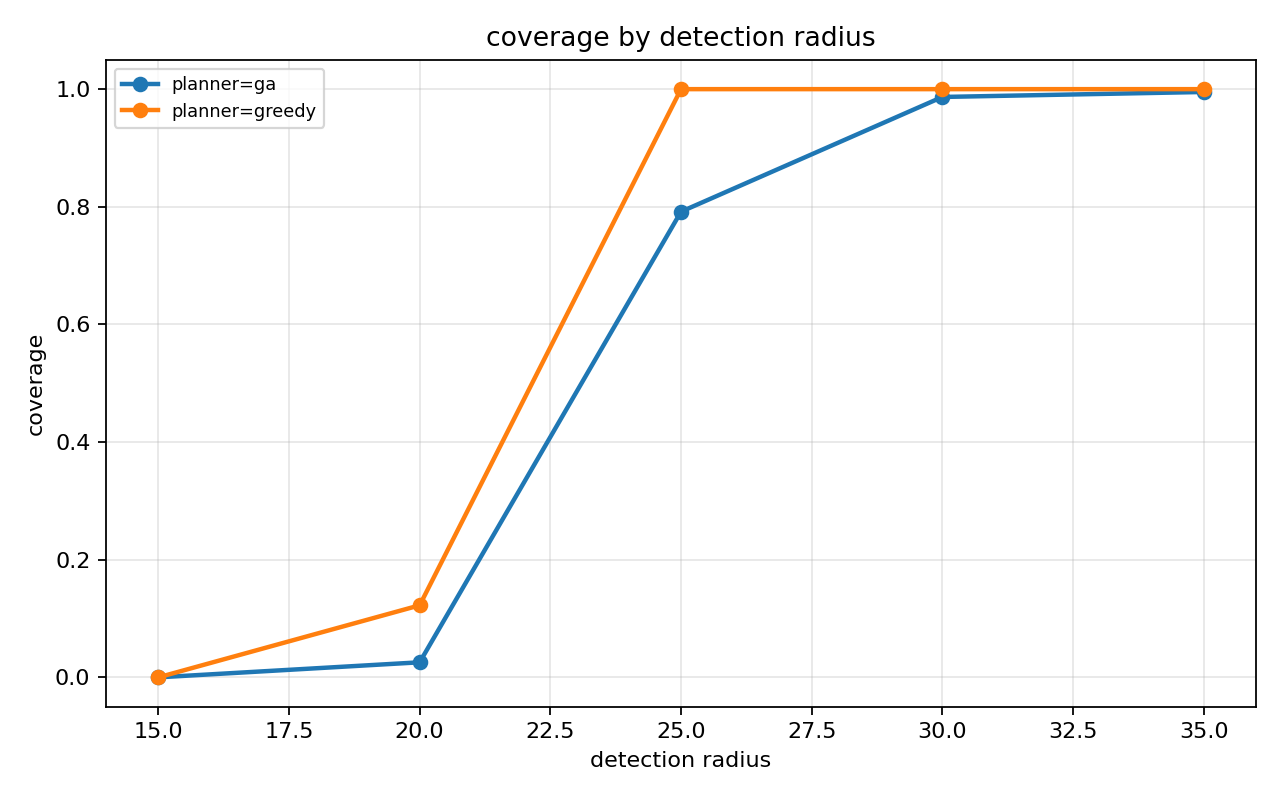
\includegraphics[width=0.9\textwidth]{../../results/experiments/detection_radius_study/plots/line_coverage_by_detection_radius_by_planner.png}
    \caption{Coverage as a function of detection radius for the greedy planner and genetic algorithm.}
    \label{fig:detection-radius-coverage}
\end{figure}

\begin{figure}[H]
    \centering
    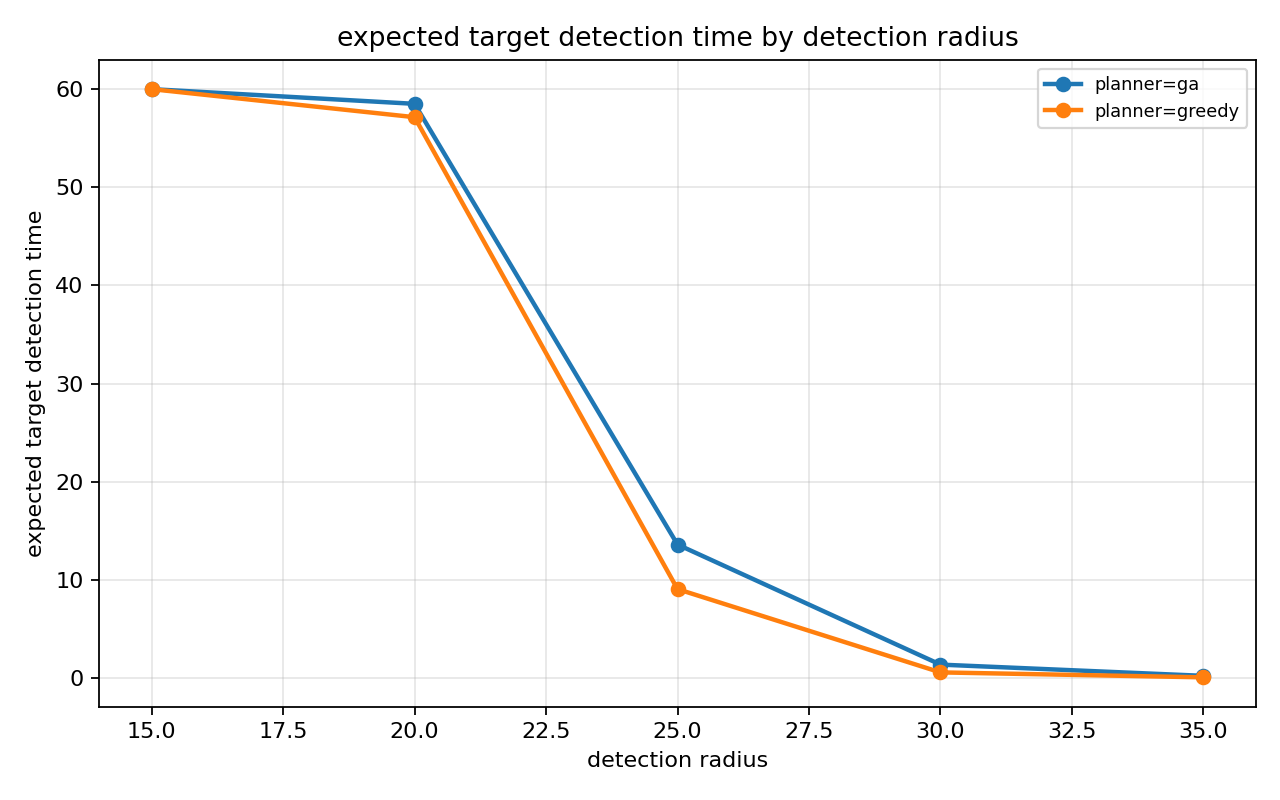
\includegraphics[width=0.9\textwidth]{../../results/experiments/detection_radius_study/plots/line_expected_target_detection_time_by_detection_radius_by_planner.png}
    \caption{Expected target detection time as a function of detection radius. Lower values indicate faster expected target discovery.}
    \label{fig:detection-radius-expected-time}
\end{figure}

\begin{figure}[H]
    \centering
    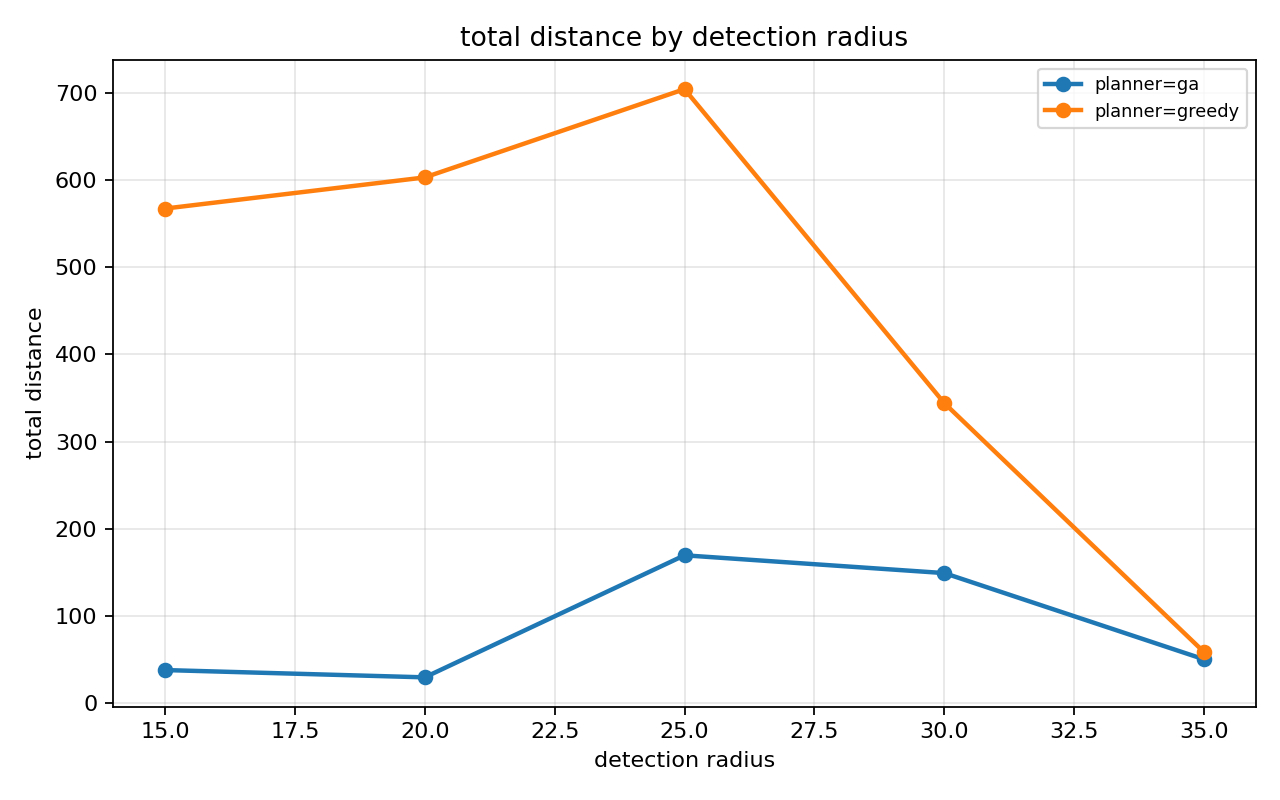
\includegraphics[width=0.9\textwidth]{../../results/experiments/detection_radius_study/plots/line_total_distance_by_detection_radius_by_planner.png}
    \caption{Total trajectory distance generated for different detection radius values.}
    \label{fig:detection-radius-distance}
\end{figure}

\begin{figure}[H]
    \centering
    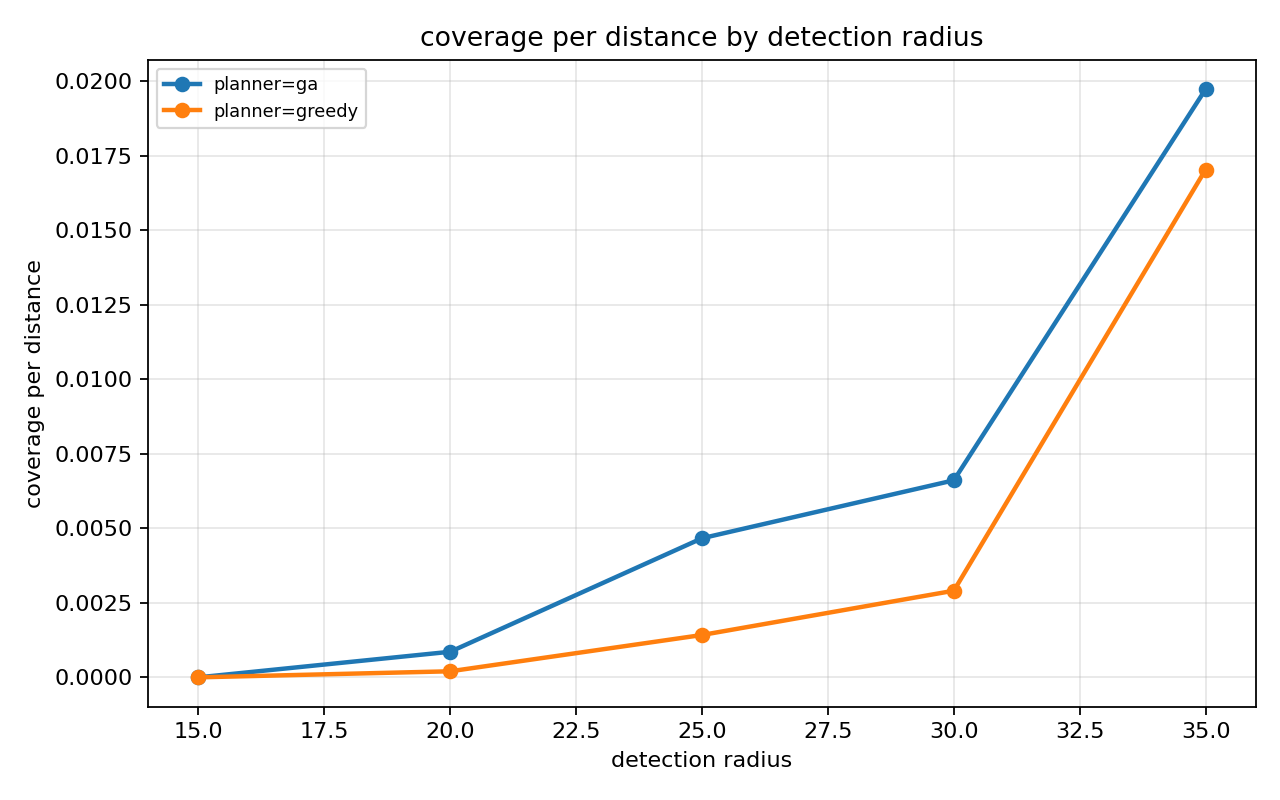
\includegraphics[width=0.9\textwidth]{../../results/experiments/detection_radius_study/plots/line_coverage_per_distance_by_detection_radius_by_planner.png}
    \caption{Coverage per travelled distance for different detection radius values.}
    \label{fig:detection-radius-efficiency}
\end{figure}

\subsection{Fleet size study}

The fleet size experiment evaluates how the number of drones affects mission
performance. Increasing the number of drones generally improves parallelism:
several areas can be searched at the same time, and high-probability regions can
be reached faster.

However, the improvement is not necessarily linear. When the number of drones
becomes large compared to the size of the search area, additional drones may
produce redundant coverage. This effect is visible in metrics such as
\texttt{coverage\_per\_distance}, where more drones can increase total travelled
distance without providing proportional improvement in coverage.
The generated comparison plots for this experiment are presented in
Figures~\ref{fig:drones-count-coverage}--\ref{fig:drones-count-efficiency}.

\begin{figure}[H]
    \centering
    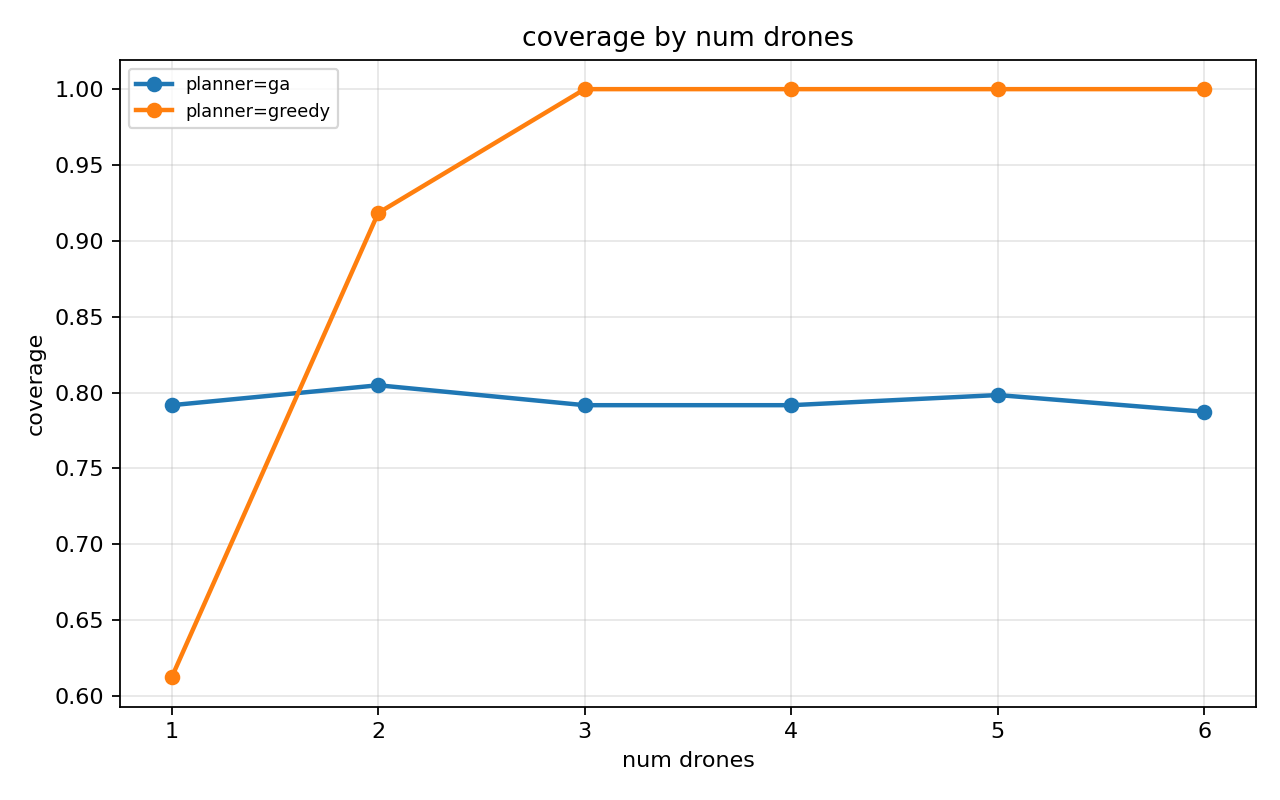
\includegraphics[width=0.9\textwidth]{../../results/experiments/drones_count_study/plots/line_coverage_by_num_drones_by_planner.png}
    \caption{Coverage as a function of the number of drones for the greedy planner and genetic algorithm.}
    \label{fig:drones-count-coverage}
\end{figure}

\begin{figure}[H]
    \centering
    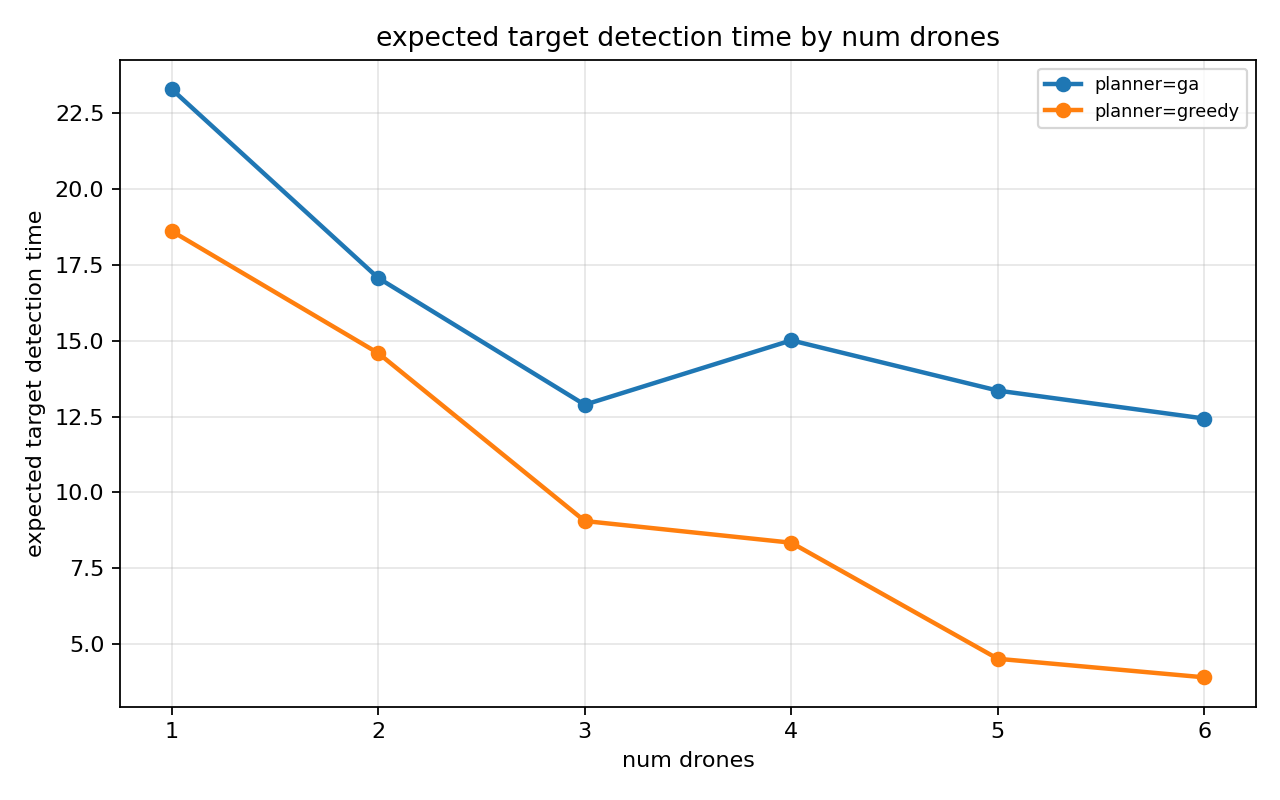
\includegraphics[width=0.9\textwidth]{../../results/experiments/drones_count_study/plots/line_expected_target_detection_time_by_num_drones_by_planner.png}
    \caption{Expected target detection time as a function of the number of drones. Lower values indicate faster expected target discovery.}
    \label{fig:drones-count-expected-time}
\end{figure}

\begin{figure}[H]
    \centering
    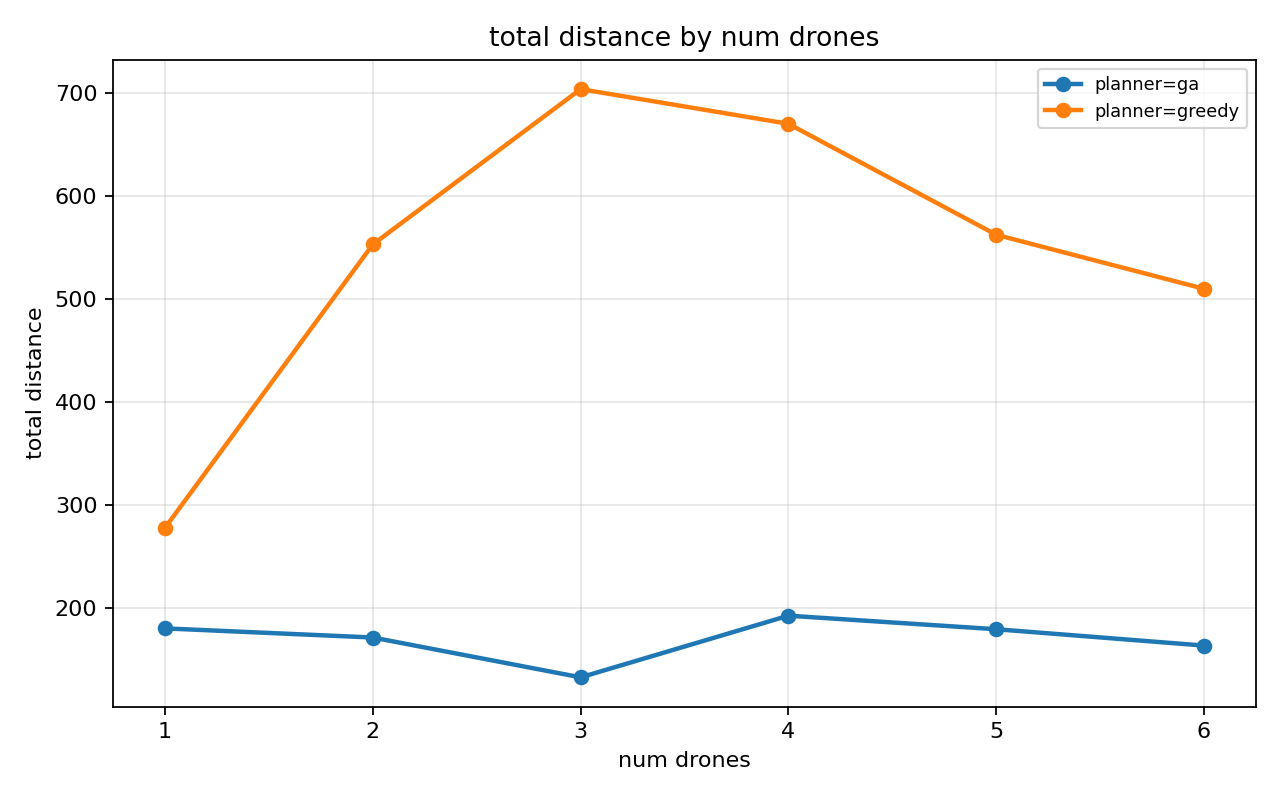
\includegraphics[width=0.9\textwidth]{../../results/experiments/drones_count_study/plots/line_total_distance_by_num_drones_by_planner.png}
    \caption{Total trajectory distance generated for different fleet sizes.}
    \label{fig:drones-count-distance}
\end{figure}

\begin{figure}[H]
    \centering
    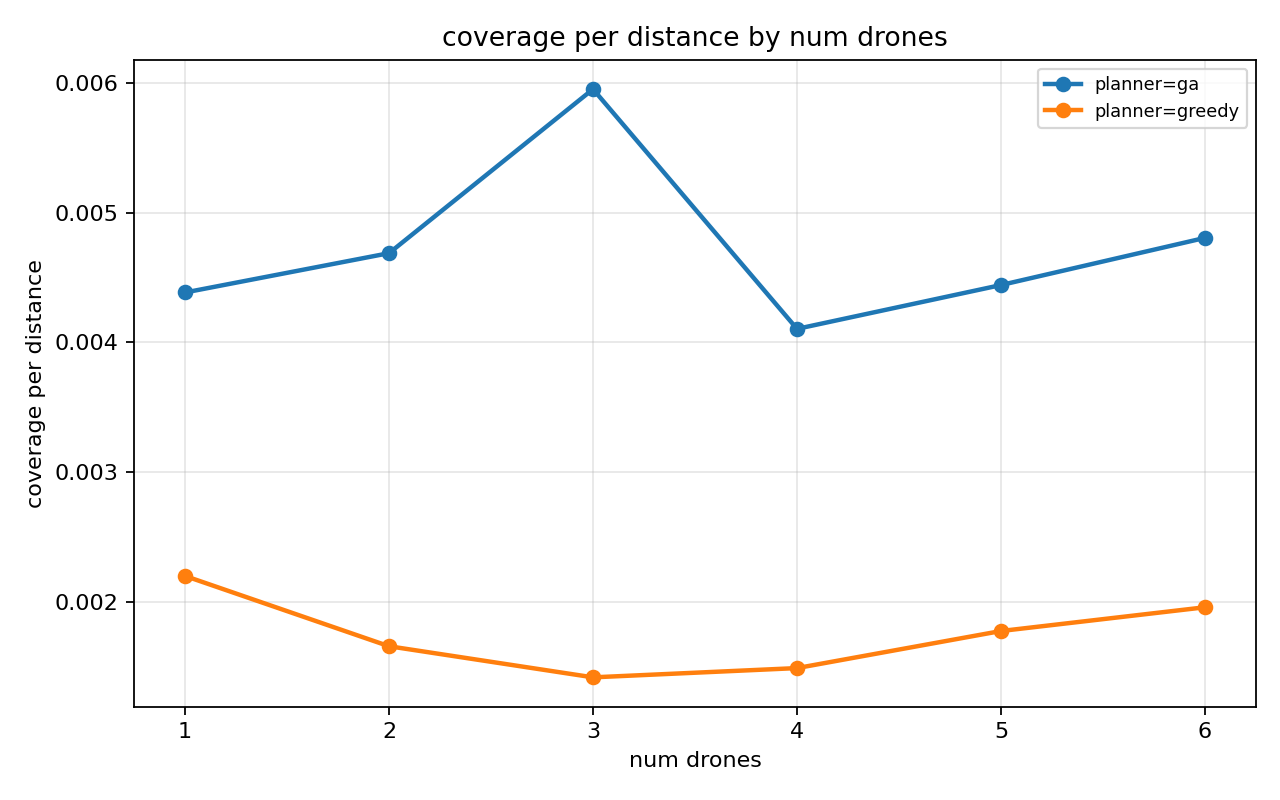
\includegraphics[width=0.9\textwidth]{../../results/experiments/drones_count_study/plots/line_coverage_per_distance_by_num_drones_by_planner.png}
    \caption{Coverage per travelled distance for different fleet sizes.}
    \label{fig:drones-count-efficiency}
\end{figure}

\subsection{Time budget study}

The time budget experiment measures how mission duration affects the quality of
planned trajectories. A short time budget limits the number of observation
points that can be reached, especially in terrain where line-of-sight
constraints require indirect movements.

As the time budget increases, both planners can generate longer trajectories and
cover more terrain cells. The expected target detection time usually decreases
because high-probability regions can be reached earlier or more reliably.
However, after the most relevant regions are covered, additional time may yield
only marginal improvement.

\subsection{Deployment pattern study}

The deployment pattern experiment compares circular and line-based starting
positions. The initial arrangement of drones affects the first observed cells
and the travel time required to reach important regions.

A circular deployment may provide better spatial distribution around the search
area, while a line deployment can be useful when the expected search direction
or terrain structure is known. The results can therefore be interpreted as a
measure of how sensitive the planning methods are to initial conditions.

\subsection{Probability map and terrain difficulty studies}

The probability map study compares a uniform distribution with a hotspot
distribution. In a uniform map, every region has similar importance, so planners
are encouraged to spread coverage more evenly. In a hotspot map, high-probability
regions dominate the expected detection time, and efficient planners should
prioritize those areas.

The terrain difficulty study evaluates the influence of terrain geometry. Flat
terrain reduces line-of-sight restrictions and makes sensor range the dominant
detection limitation. Hilly or mountainous terrain introduces occlusions, which
can make nearby cells invisible and require additional observation points.

\subsection{Discussion of results}

The experimental results confirm that terrain-aware visibility is a significant
factor in multi-drone search planning. Increasing the detection radius improves
results, but it does not completely eliminate the effect of terrain occlusions.
In difficult terrain, appropriate placement of observation points remains
important.

The greedy planner provides fast and interpretable solutions. It performs well
when local gains correspond closely to global mission quality. Its main
limitation is its myopic behavior: once it selects locally attractive moves, it
does not reconsider earlier decisions.

The genetic algorithm explores a broader solution space and can find compact
trajectory sets with good coverage. At the same time, it is more computationally
expensive and sensitive to configuration parameters such as population size,
mutation rate, chromosome length, and number of generations.

The expected target detection time metric is particularly useful because it
connects coverage quality with mission urgency. A trajectory that eventually
covers many cells may still be less useful if high-probability regions are
visited late. Therefore, this metric provides a more mission-oriented evaluation
than coverage alone.

\section{\SectionTitleSummary}

The project addressed the problem of coordinating multiple drones in a
search-and-rescue mission over non-flat terrain. The target location was modeled
probabilistically, and detection was constrained by both sensor radius and
terrain-dependent line-of-sight visibility.

The implemented system includes terrain generation, probability map generation,
visibility analysis, detection checking, greedy trajectory planning, genetic
algorithm optimization, batch experiment execution, plot generation, and Webots
visualization.

The main conclusions are as follows:
\begin{itemize}
    \item terrain geometry has a strong influence on detection capability because line-of-sight restrictions can prevent observation even when the target is close to a drone,
    \item the detection-radius plots show that sensor range is one of the most influential mission parameters: for the smallest tested radius both planners remained close to the full mission time budget, while larger radii strongly improved coverage and reduced expected target detection time,
    \item for larger detection radii, both planners reached high coverage while requiring fewer effective observation moves, which shows that better sensing can also reduce unnecessary travel,
    \item the fleet-size plots show that adding drones improves parallel search and reduces expected detection time, especially for the greedy planner, but the improvement saturates after full or near-full coverage is reached,
    \item the coverage-per-distance plots show that more drones do not automatically mean better efficiency, because additional drones can increase total travelled distance or create redundant coverage,
    \item the greedy planner is fast, interpretable, and effective as a baseline method; in the experiments it achieved strong coverage, but often at the cost of longer total trajectories,
    \item the genetic algorithm usually produced shorter and more distance-efficient trajectories, but its results were less stable in single runs due to the stochastic nature of evolutionary optimization; repeated runs and confidence intervals would be needed for stronger statistical conclusions,
    \item expected target detection time is a better mission-oriented metric than coverage alone, because it captures not only whether important regions are observed, but also how quickly high-probability target locations are reached,
    \item no single metric is sufficient on its own: coverage, expected detection time, total distance, and coverage per distance should be analyzed together to understand the practical quality of a multi-drone search plan.
\end{itemize}

The current implementation provides a functional simulation and evaluation
framework, but several limitations remain. The drone motion model is simplified,
the trajectories are planned offline, and the Webots execution layer does not
include realistic flight dynamics or collision avoidance. The genetic algorithm
also uses a relatively simple representation and genetic operators.

Future work may include online replanning, dynamic probability updates after
partial observations, more realistic UAV dynamics, collision avoidance,
communication constraints, larger terrain datasets, and more advanced
evolutionary or learning-based planning methods. In addition, future
experiments should include repeated genetic algorithm runs with different
random seeds, confidence intervals for the plotted metrics, and larger
benchmark scenarios. This would make it possible to distinguish systematic
planner behavior from stochastic variation caused by evolutionary search.

Overall, the obtained results show that multi-drone search planning can benefit
from combining probabilistic target modeling with terrain-aware visibility
analysis. The developed framework makes it possible to compare planning
strategies and evaluate how mission parameters influence search effectiveness.


%%%%%%%%%%%%%%%%%%%%%%%%%%%%%%%%%%%%%%%%%%%%%%%%%%%%%%%%%%%%%%%%%%%%%%%%%%%%%%%
\printbibliography

%%%%%%%%%%%%%%%%%%%%%%%%%%%%%%%%%%%%%%%%%%%%%%%%%%%%%%%%%%%%%%%%%%%%%%%%%%%%%%%
\end{document}
